\documentclass{article}
\usepackage[utf8]{inputenc} % allow utf-8 input
\usepackage[T1]{fontenc}    % use 8-bit T1 fonts
\usepackage{hyperref}       % hyperlinks
\usepackage{url}            % simple URL typesetting
\usepackage{booktabs}       % professional-quality tables
\usepackage{amsfonts}       % blackboard math symbols
\usepackage{nicefrac}       % compact symbols for 1/2, etc.
\usepackage{microtype}      % microtypography
\usepackage{graphicx}
\usepackage{ifthen}
\usepackage{tikz}
\usepackage{eso-pic}
\usepackage{color}
\usepackage{float}
\usepackage{multicol}
\usepackage{setspace}
\usepackage{mathptmx}
%\usepackage{mathpazo}
\usepackage[theorems]{tcolorbox}
\usepackage{mdframed}
\usepackage{amsmath,amsthm,amssymb,mathtools,flexisym,bbm}
\usepackage{xcolor,paralist,hyperref,fancyhdr,etoolbox}
\usepackage{mathrsfs}
\usepackage{pgfplots}
\usepackage{xcolor}
\usepackage[shortlabels]{enumitem}
\usepackage{algorithm}
\usepackage[noend]{algpseudocode}
\usepackage{cite}
\usepackage{multirow}
\usepackage[font=scriptsize]{caption}
\usepackage{subcaption}
\usepackage{comment}
\usepackage{xspace}
\usepackage{environ}
\usepackage{longtable}
% \baselineskip=16pt
\usepackage{indentfirst,csquotes}
\usepackage{array}


\usepackage[margin=1in]{geometry}

\newtheorem{theorem}{Theorem}[section]
\newtheorem{definition}[theorem]{Definition}
\newtheorem{example}[theorem]{Example}
\newtheorem{lemma}[theorem]{Lemma}
\newtheorem{proposition}[theorem]{Proposition}
\newtheorem{corollary}[theorem]{Corollary}
\newtheorem{conjecture}[theorem]{Conjecture}
\newtheorem*{claim}{Claim}
\newtheorem{remark}[theorem]{Remark}


\newcolumntype{H}{>{\setbox0=\hbox\bgroup}c<{\egroup}@{}}
\hypersetup{colorlinks=true, linkcolor=black, filecolor=black, urlcolor=black }
% \def\proof{\noindent {\it Proof. $\, $}}
% \def\endproof{\hfill $\Box$ \vskip 5 pt }


%Define some symbols
\DeclarePairedDelimiter\abs{\lvert}{\rvert}%
\DeclarePairedDelimiter\norm{\lVert}{\rVert}%

\newcommand{\PI}{\textbf{Phase~I}\xspace}
\newcommand{\PII}{\textbf{Phase~II}\xspace}
\newcommand{\N}{\mathbb{N}}
\newcommand{\F}{\mathbb{F}}
\newcommand{\Z}{\mathbb{Z}}
%\newcommand{\R}{\mathbb{R}}
\newcommand{\R}{\mathbb{R}}
\newcommand{\Q}{\mathbb{Q}}
\newcommand{\E}{\mathbb{E}}
\newcommand{\B}{\mathbb{B}}
\newcommand{\C}{\mathbb{C}}
\newcommand{\T}{\mathbb{T}}
\newcommand{\barS}{\bar{S}}
\newcommand{\calU}{\mathcal{U}}
\newcommand{\tr}{\operatorname{tr}}
\newcommand{\Diag}{\operatorname{Diag}}
\newcommand{\TriDiag}{\operatorname{TriDiag}}
\newcommand{\tridiag}{\operatorname{tridiag}}
\newcommand{\BiDiag}{\operatorname{BiDiag}}
\newcommand{\bidiag}{\operatorname{bidiag}}
\newcommand{\diag}{\operatorname{diag}}
\newcommand{\vectorize}{\operatorname{vec}}
\newcommand{\adj}{\operatorname{adj}}
\newcommand{\svec}{\operatorname{svec}}
\newcommand{\symm}{\mathbb{S}}
\renewcommand{\symm}{\mathbb{S}}
\newcommand{\PSD}{\mathbb{S}_{+}}
\newcommand{\PD}{\mathbb{S}_{++}}
\newcommand{\rank}{\operatorname{rank}}
\newcommand{\proj}{\mathbf{P}}
\newcommand{\algo}{{\color{red}\emph{algorithm-name} }}
\newcommand{\calV}{\mathcal{V}}
\newcommand{\SDP}{\text{SDP}}
\newcommand{\LP}{\text{LP}}
\DeclareMathOperator{\Null}{Null}
\DeclareMathOperator{\range}{Range}
\DeclareMathOperator{\rint}{rint}
\DeclareMathOperator{\dom}{dom}
\DeclareMathOperator{\row}{row}
\DeclareMathOperator{\spn}{span}
\DeclareMathOperator{\conv}{conv}
\DeclareMathOperator{\SM}{SparseMat}
\DeclareMathOperator{\CLQ}{CLQ}
\DeclareMathOperator{\thbody}{TH}
\DeclareMathOperator{\STAB}{STAB}
\DeclareMathOperator{\pes}{pes}

\newcommand{\st}{\text{s.t.}}

\renewcommand{\algorithmicrequire}{\textbf{Input:}}
\renewcommand{\algorithmicensure}{\textbf{Output:}}

\renewcommand{\subset}{\subseteq}
\renewcommand{\supset}{\supseteq}
\DeclareMathOperator*{\argmax}{arg\,max}
\DeclareMathOperator*{\argmin}{arg\,min}
% --- compact multiline displays ---
\allowdisplaybreaks            % allow page breaks inside align
\setlength{\jot}{2pt}          % row spacing in align/aligned
\AtBeginDocument{%
  \setlength{\abovedisplayskip}{4pt}
  \setlength{\belowdisplayskip}{4pt}
  \setlength{\abovedisplayshortskip}{4pt}
  \setlength{\belowdisplayshortskip}{4pt}
}


\tikzset{every picture/.style={line width=0.75pt}} %set default line width to 0.75pt        
%\captionsetup{skip=2pt}
\captionsetup[subfigure]{aboveskip=0pt}
\setlength{\textfloatsep}{5pt}
\setlength{\intextsep}{5pt}  

\newcommand{\dcnote}[1]{{\color{blue} DC: #1}}
\newcommand{\rgnote}[1]{{\color{magenta} RG: #1}}
\newcommand{\atnote}[1]{{\color{brown} AT: #1}}


\title{Dynamic Interval Scheduling with Random Start and End Times\thanks{Partially funded by the U.S. Office of Naval Research, N00014-23-1-2631.}} %%%%%%%%%%%%
\author{Rui Gong\thanks{
Corresponding author (rgong44@gatech.edu)\\
\indent~~ Georgia Institute of Technology, Atlanta, GA 30332, USA\\
\indent~~ The authors' work was partially funded by the U.S.\ Office of Naval Research, N00014-23-1-2631.} \and 
% Diego Cifuentes \and 
Alejandro Toriello}

\begin{document}
\maketitle
\begin{abstract}
We study sequential interval scheduling when task start and end times are random.
The set of tasks and their weights are known in advance, while each task's start and end times are drawn from known discrete distributions and revealed only upon commitment;
this also eliminates tasks that conflict with the committed task, and remaining tasks are those that do not conflict. 
%Tasks conflicting with already committed tasks are discarded, and remaining tasks update their distributions accordingly.
The objective is to maximize the expected weight of a conflict-free schedule.
We propose two models that differ in how conflicts are enforced, develop LP relaxations and bounds for each, and present a computational study.
\end{abstract}

\section{Introduction}
The \emph{interval scheduling problem} is classical in operations research, industrial engineering and computer science.
It considers a set of tasks $N:=[n] = \{1, \dotsc, n\}$ and consecutive time slots $M:=[m]$.
Each task is represented by an interval $[s_i,e_i]$ describing the time slots it occupies if scheduled.
The \emph{maximum interval scheduling problem} seeks a set of pairwise nonoverlapping intervals (a schedule) of maximum total weight.
When all tasks have the same weight, the greedy rule that repeatedly selects the earliest-ending task and discards conflicts is optimal;
the weighted version is also solvable in $\Theta(n)$ time \cite{Kleinberg+Tardos:06a}.

An \emph{interval graph} is an undirected graph representing intervals on a line, where each vertex corresponds to an interval and an edge connects two vertices if their intervals overlap.
Thus a feasible schedule corresponds exactly to an independent set of the associated interval graph.
Since interval graphs are perfect, the maximum interval scheduling problem can be represented by the clique LP pair of the interval graph $G=(N,E)$,
\begin{multicols}{2}
    \noindent
    \begin{align}
\label{LP-P}
\tag{LP-P}
\begin{split}
    \max_{x\geq 0}\quad &w^\top x\\
    \st\quad &\sum_{i\in C}x_i\leq 1, \forall C\in\mathcal{C}(G)
\end{split}
\end{align}
\columnbreak
\begin{align}
\label{LP-D}
\tag{LP-D}
\begin{split}
    \min_{\mu\geq0}\quad &\sum_{C\in\mathcal{C}(G)}\mu_C\\
    \text{s.t.}\quad &\sum_{C\ni i}\mu_C\geq w_i,~\forall i\in N,
\end{split}
\end{align}
\end{multicols}
\noindent
where $\mathcal{C}(G)$ is the set of all maximal cliques of $G$.
\eqref{LP-P} formulates the maximum independent set problem and \eqref{LP-D} formulates the corresponding minimum clique cover problem.
For arbitrary perfect graphs, \eqref{LP-P} and \eqref{LP-D} are tight formulations, but not guaranteed to be solvable in polynomial time because there are possibly exponentially many maximal cliques.
In contrast, in interval graphs the number of maximal cliques is at most $\min\{m, n\}$.
Thus the deterministic maximum interval scheduling problem can be solved efficiently either directly or via these LP relaxations.
Our goal is to extend this setting to incorporate uncertainty and sequential decisions while retaining tractable relaxations and algorithms.

Several stochastic interval scheduling models have been studied.
A classical one is \emph{online interval scheduling}~\cite{Lipton1994OnlineIS}, where intervals of fixed length are presented to the scheduler in the order of their start times and must be accepted or rejected irrevocably.
The objective is to maximize total weight while maintaining feasibility.
Recent work includes online interval scheduling with predictions of upcoming intervals~\cite{boyar2025onlineintervalschedulingpredictions} and models that allow overlaps but maximize a satisfaction objective~\cite{KOBAYASHI2020673}.
Other variants include interval scheduling with random delays~\cite{BRANDA2024106542} and settings where tasks may depart unexpectedly and service times are stochastic~\cite{xu2024stochasticschedulingabandonmentsgreedy}.

We study the setting where the set of tasks and their weights are known in advance but task start and end times are random.
The scheduler commits to tasks sequentially, learns realized intervals as tasks are committed, and seeks to maximize the expected total weight.

\section{Dynamic Scheduling with Random Start and End Times}
%We introduce the following model.
We again let $M=[m]$ be the set of slots, $N=[n]$ the set of tasks, and $w\in\R_{+}^{N}$ the task weights. 
For each task $i\in N$, let $D_i^s,D_i^e$ be the independent discrete distributions of $i$'s start and end times, and denote $S_i,E_i\subseteq M$ as their supports.
We assume $\max S_i\leq \min E_i$ and define $D:=\{D_i^*:*\in\{s,e\},i\in N\}$.
When task $i$ is scheduled, its start and end times $s_i,e_i$ are realized according to $D_i^s$ and $D_i^e$. 
For each remaining task $j$, we compute the probability $p_{ij}$ that it conflicts with $i$ based on $s_i$, $e_i$, $D_j^s$ and $D_j^e$, and draw $B_{ij}\sim\operatorname{Bernoulli}(p_{ij})$.
If $B_{ij}=1$, task $j$ is deleted; otherwise, it remains available and its distributions are updated to condition on the slots occupied by $i$, $[s_i, e_i]$. 
The goal is to schedule tasks sequentially and maximize the expected total weight of scheduled tasks.
We call this problem \emph{dynamic scheduling with random start and end times (DSRSE)}.

DSRSE can be formulated as a dynamic program with the Bellman recursion
\[
%\max_{\pi\in \Pi}\E_\pi\left[V^\pi(N,M,w,D)\right];\quad~ 
V^*(N,M,w,D):=\max_i\{w_i+\E[V^*(N',M',w,D')]\},
\]
where %$\Pi$ is the set of all policies and $V^\pi(N,M,w,D)$ is a random variable representing the total weight of scheduled tasks under policy $\pi\in\Pi$.
$V^*$ is the optimal value function and $N',M',w,D'$ are the random variables representing the resulting state after scheduling task $i$.
Like many dynamic programming problems, this problem has exponentially many states and each state has $O(n)$ actions, so it is unreasonable to solve it directly;
moreover, the problem is NP-hard.
\begin{proposition}
    DSRSE is NP-hard.
\end{proposition}
\begin{proof}
    Suppose there are $n+1$ tasks and $2n$ slots.
    Let $0$ be a task taking positions $1,\ldots,n$ with probability $1$, and task $i$ taking position $i$ with probability $p_i$ and $n+i$ with probability $(1-p_i)$.
    Then this problem is equivalent to the dynamic maximum stable set problem over a star graph, where $0$ is the center;
    this problem is NP-hard~\cite{DNP}.
\end{proof}
\begin{example}
\label{eg:1}
    Consider an instance with $N=[2],M=[3]$, and unit weights, where $D_1^s=\mathbbm{1}_{\{1\}},D_1^e=\mathbbm{1}_{\{2\}}$, $D_2^s=U(\{2,3\}),D_2^e=\mathbbm{1}_{\{3\}}$.
If the scheduler commits to task $1$ first, then task $1$ occupies $[1,2]$.
%
If task $1$ is scheduled, task $2$ has a probability of $1/2$ of conflicting and $1/2$ of remaining.
%Flip a fair coin.
If it remains, task $2$'s distributions are updated to condition on the fact that it does not conflict with task 1: $D_2^s=\mathbbm{1}_{\{3\}},D_2^e=\mathbbm{1}_{\{3\}}$.
On the other hand, if task $2$ is scheduled first and its start time realizes to $2$, task $1$ is deleted; if it realizes to $3$, task $1$ remains.
\end{example}
When $s_i,e_i$ are deterministic for every task, DSRSE reduces to the maximum independent set problem of the corresponding interval graph.
As discussed above, it can be represented by~\eqref{LP-P} and~\eqref{LP-D}, so the deterministic problem can be solved efficiently via these LP relaxations.
For an interval graph, maximal cliques are elements of $M$, so the constraint $\sum_{i\in C}x_i\leq 1,\forall C\in\mathcal{C}(G)$ in~\eqref{LP-P} simply enforces that each slot is occupied by at most one task.
We consider analogous constraints for DSRSE.


\subsection{Relaxations}
For DSRSE, consider $P^s,P^e,P^o\in\R^{n\times m}$, where $P_{ik}^s,P_{ik}^e,P_{ik}^o$ are the probabilities that task $i$ starts at, ends at, and occupies slot $k$, respectively.
Let $T=[\min\{m,n\}]$ be the stages of the dynamic program.
For any policy, let $x_{ik}^{ts},x_{ik}^{te},x_{ik}^{to}$ be the probabilities that $i$ is scheduled and starts at, ends at, or occupies slot $k$ at stage $t$, respectively.
Let $x_i^t = \sum_{k=1}^m x_{ik}^{ts}=\sum_{k=1}^{m} x_{ik}^{te}$ be the probability of scheduling $i$ at stage $t$.
The objective can then be written as $ \max \sum_{t}\sum_i w_i\, x_{i}^t $.
Analogous to the deterministic case, we impose that the probability a slot is occupied is at most $1$.
We relax DSRSE to
\begin{align*}
    \max~&\sum_{t}\sum_i w_i\, x_{i}^{t}\\
    &x_i^t =\sum_{k=1}^{m}x_{ik}^{ts}=\sum_{k=1}^{m}x_{ik}^{te}, \forall i,\forall t\in T\\
    &x_{ik}^{ts}=0,\forall t\in T,\forall k\notin S_i\\
    &x_{ik}^{te}=0,\forall t\in T,\forall k\notin E_i\\
    &\sum_t\sum_i x_{ik}^{to}\leq 1,\forall k\in M\\
    &\sum_{t}x_{ik}^{ts}\leq P_{ik}^{s},~\sum_{t}x_{ik}^{te}\leq P_{ik}^{e}~\forall i\in N,\forall k\in M\\
    &0\leq x_{i}^{t}, x_{ik}^{ts},x_{ik}^{te}, x_{ik}^{to},
\end{align*}
where $x_{ik}^s:=\sum_{t}x_{ik}^{ts}\leq P_{ik}^s$ indicates that the probability of $i$ being scheduled and starting at $k$ is at most the marginal probability $P_{ik}^s$, and similarly for $x_{ik}^{e}:=\sum_t x_{ik}^{te}\leq P_{ik}^e$.
For each $k\in M$, we can rewrite $\sum_t\sum_i x_{ik}^{to}\leq 1$ as
\begin{align}
%\begin{split}
    &\sum_{t}\sum_{i}x_{ik}^{to}\notag \\
=&\sum_{t} \left(\sum_{i,a_i\leq k\leq b_i}x_{ik}^{to}+\sum_{i,c_i\leq k\leq d_i}x_{ik}^{to}+\sum_{i,b_i< k< c_i}x_{ik}^{to}\right) \notag \\
= &\sum_{t} \left(\sum_{i,a_i\leq k\leq b_i-1}\sum_{\ell = a_i}^{k}x_{i\ell}^{ts}+\sum_{i,c_i+1\leq k\leq d_i}\sum_{\ell =k}^{d_i}x_{i\ell}^{te}+\sum_{i,b_i\leq k\leq c_i}x_{i}^{t}\right)  \notag \\
=&\sum_{t}\sum_{i, b_i\leq k\leq c_i} x_i^t+\sum_t \left(\sum_{i,a_i\leq k\leq b_i-1}\sum_{\ell = a_i}^{k}x_{i\ell}^{ts}+\sum_{i,c_i+1\leq k\leq d_i}\sum_{\ell =k}^{d_i}x_{i\ell}^{te}\right)\notag \\
\leq &1,  \label{eq:1}
%\end{split}
\end{align}
where $a_i:=\min\{k:k\in S_i\},b_i:=\max\{k:k\in S_i\},c_i:=\min\{k:k\in E_i\},d_i:=\max\{k:k\in E_i\}$.
The first equality comes from the fact that the probability $i$ occupies a slot $k$ not in $S_i\cup E_i\cup (b_i,c_i)$ is $0$.
For the second equality, by definition, any $k\in [b_i,c_i]$ is always occupied by $i$ if it is scheduled, so $x_{ik}^{to}=x_{i}^t$; for $k\in[a_i,b_i)$, the probability of $i$ being scheduled and occupying $k$ at $t$ is equivalent to the probability of $i$ being scheduled and starting at or before $k$ at $t$, and similarly for the ending slots.
The third equality is derived by rearranging terms.
Since $\sum_{i,a_i\leq k\leq b_i-1}\sum_{\ell = a_i}^{k}x_{i\ell}^{ts} = \sum_{i,a_i\leq k\leq b_i-1}(x_i^t-\sum_{\ell = k+1}^{b_i}x_{i\ell}^{ts})$, and similarly for $x_{i\ell}^{te}$, we have for every $k\in M$,
\begin{equation}
    \label{eq:2}
    \sum_{t}\left(\sum_{i, a_i\leq k\leq d_i} x_i^t-\sum_{i,a_i\leq k\leq b_i}\sum_{\ell = k+1}^{b_i}x_{i\ell}^{ts}-\sum_{i,c_i\leq k\leq d_i}\sum_{\ell =c_i}^{k-1}x_{i\ell}^{te}\right)\leq 1.
\end{equation}
Then we have the following primal-dual pair:
% \begin{multicols}{2}
% \noindent
    \begin{align*}
    \label{DLP-P}
    \tag{DLP-P}
    \begin{split}
            \max_{x\geq 0}~&\sum_{t}\sum_i w_i\, x_{i}^{t}\\
    &x_i^t =\sum_{k=1}^{m}x_{ik}^{ts}=\sum_{k=1}^{m}x_{ik}^{te}, \forall i\in N,\forall t\in T\\
    &x_{ik}^{ts}=0,\forall t\in T,\forall k\notin [a_i,b_i]\\
    &x_{ik}^{te}=0,\forall t\in T,\forall k\notin [c_i,d_i]\\
& \sum_{t}\biggl(\sum_{i, a_i\leq k\leq d_i} x_i^t 
  - \sum_{i,a_i\leq k\leq b_i}\sum_{\ell = k+1}^{b_i}x_{i\ell}^{ts} - \sum_{i,c_i\leq k\leq d_i}\sum_{\ell =c_i}^{k-1}x_{i\ell}^{te}\biggr) \leq 1,
  ~\forall k\in M \\
    &\sum_{t}x_{ik}^{ts}\leq P_{ik}^{s},~\sum_{t}x_{ik}^{te}\leq P_{ik}^{e},\forall i\in N,\forall k\in M\\
    \end{split}
\end{align*}
% \columnbreak
\begin{align*}
\label{DLP-D}
    \tag{DLP-D}
\begin{split}
\min_{\mu,\nu,u\geq 0,y,z}\quad 
& \sum_{r=1}^{m} \mu_r
  + \sum_{i=1}^{n}\sum_{k\in S_i} P^s_{ik}\,\nu^s_{ik}
  + \sum_{i=1}^{n}\sum_{k\in E_i} P^e_{ik}\,\nu^e_{ik}
  + \sum_{i=1}^{n}\sum_{t=1}^{T} u_{it}\\
\text{s.t.}\quad 
& y_{it} + z_{it} + u_{it} + \sum_{r=a_i}^{d_i} \mu_r \geq w_i,
\forall\, i\in N,\ \forall\, t\in T, \\
& -y_{it} -\sum_{r=a_i}^{k-1} \mu_r+\nu^s_{ik}\geq0,\forall\, i\in N,\ \forall\, t\in T,\ \forall\, k\in S_i, \\
& -z_{it}-\sum_{r=k+1}^{d_i} \mu_r+\nu^e_{ik}\geq 0,\forall\, i\in N,\ \forall\, t\in T,\ \forall\, k\in E_i.
\end{split}
\end{align*}
% \end{multicols}
\noindent
By setting $y,z, u$ to $0$,~\eqref{DLP-D} is equivalent to,
\begin{align*}
\tag{LP-Dpes}
\label{LP-Dpes}
\min_{\mu,u\geq 0}\quad 
& \sum_{r=1}^{m} \mu_r
  + \sum_{i=1}^{n}\sum_{k\in S_i} P^s_{ik}\,\sum_{r=a_i}^{k-1} \mu_r
  + \sum_{i=1}^{n}\sum_{k\in E_i} P^e_{ik}\,\sum_{r=k+1}^{d_i} \mu_r\\
\text{s.t.}\quad 
&\sum_{r=a_i}^{d_i} \mu_r \geq w_i,
~\forall\, i\in N.
\end{align*}
Consider the pessimistic interval graph $G_{\pes}$, where each task $i$ occupies $[a_i,d_i]$, the widest possible interval, and the corresponding LP \eqref{LP-D} defined on $G_{\pes}$; 
let $\mu_{\pes}$ be its optimal solution, and $\alpha_{\pes}:=\alpha(G_{\pes})=\sum_{r}[\mu_{\pes}]_r$ its optimal value.
Since $\mu = \mu_{\pes}, y=z=u=0$ is feasible for \eqref{DLP-D}, the optimal value of \eqref{DLP-D}, $\alpha^*$, is at most \[\alpha_{\pes}+\sum_{i=1}^{n}\sum_{k\in S_i} P^s_{ik}\,\sum_{r=a_i}^{k-1} {[\mu_{\pes}]}_r
  + \sum_{i=1}^{n}\sum_{k\in E_i} P^e_{ik}\,\sum_{r=k+1}^{d_i} {[\mu_{\pes}]}_r,\] where
\begin{align*}
\sum_{i=1}^{n}\sum_{k\in S_i} P^s_{ik}\, \sum_{r=a_i}^{k-1}{[\mu_{\pes}]}_r = & \sum_{r}{[\mu_{\pes}]}_r\sum_{i}\sum_{k,r\in S_i, k>r}P_{ik}^s\\
=&\sum_r {[\mu_{\pes}]}_r \sum_{i\text{ s.t. }r\in S_i} (1-P_{ir}^o),
\end{align*}
%similar for the other term, we have 
and
\[\sum_{i=1}^{n}\sum_{k\in E_i} P^e_{ik}\,\sum_{r=k+1}^{d_i} {[\mu_{\pes}]}_r= \sum_{r}{[\mu_{\pes}]}_r\sum_{i\text{ s.t. }r\in E_i}(1-P_{ir}^o).\]
Thus,
\begin{align*}
\sum_r [\mu_{\pes}]_r\leq & \alpha^*\leq\sum_r [\mu_{\pes}]_r\left(1+\sum_{i\text{ s.t. }r\in S_i} (1-P_{ir}^o)+\sum_{i\text{ s.t. }r\in E_i} (1-P_{ir}^o)\right).
\end{align*}
The bound is tight when the problem is deterministic because for every $r\in M$, $\sum_{i\text{ s.t. }r\in S_i} (1-P_{ir}^o) = \sum_{i\text{ s.t. }r\in E_i} (1-P_{ir}^o) = 0$.

We conclude this section by considering the special case where tasks only occupy one slot, $ s_i = e_i $.
%If the length of each task is fixed to be $1$, that is, $s_i=e_i$, the problem is trivial.
\begin{proposition}
    If each task always occupies only a single slot, a greedy policy is optimal.
\end{proposition}
\begin{proof}
    We use an adversarial argument.
    Consider an adversary that places tasks $N$ into $[m]$ positions in advance according to their distributions $D_i^s,D_i^e$ for each $i\in N$.
    Since the length of each task is $1$, if the positions of the tasks are known, it is optimal to pick the largest weighted task of each position.
    Without loss of generality, assume the weights of the largest weighted task of each position to be $w_1\geq w_2\geq \ldots w_m\geq 0$.
    Without knowing the positions, the greedy policy would pick $w_1,w_2,\ldots, w_m$ which is equivalent to the case where positions are known.
    Thus, for any realization, the greedy policy returns the set of non-conflicting tasks with the maximum weights.
\end{proof}
\section{Conservative DSRSE}
In this section, we consider another version of DSRSE, where a task is deleted whenever it possibly conflicts with the committed tasks.

We have $M,N,w,D$, like in DSRSE. 
Once $s_i,e_i$ of a committed task are determined, for any remaining task $j$, instead of flipping a coin, we delete $j$ if any slot in its support is occupied by committed tasks; otherwise, keep $j$.
The goal remains to schedule tasks sequentially and maximize the expected total weight of scheduled tasks.
We call this problem \emph{conservative dynamic scheduling with random start and end times (CDSRSE)}.

\begin{example}
\label{eg:2}
    Consider an instance with $N=[2],M=[3]$, and unit weights, where $D_1^s=\mathbbm{1}_{\{1\}},D_1^e=\mathbbm{1}_{\{2\}}$, $D_2^s=U(\{2,3\}),D_2^e=\mathbbm{1}_{\{3\}}$.
If we commit to task $1$ first, then task $1$ occupies $[1,2]$.
For CDSRSE, task $2$ is always deleted, since position $2$ is in its support, which is now occupied by task $1$.
\end{example}
%Even CDSRSE remains NP-hard.
\begin{theorem}%[\cite{DNP}]
    CDSRSE is also NP-hard.
\end{theorem}
\begin{proof}
    As in the previous proof, consider the instance with $n+1$ tasks and $2n$ slots. 
    Task $0$ occupies slots $1,\ldots,n$ with probability $1$, and task $i$ occupies slot $i$ with probability $p_i$ and $n+i$ with probability $q_i:=1-p_i$.
    As in \cite{DNP}, any solution for this problem is determined by when to select task $0$, and what is selected before trying to select task $0$.
    Then the problem can be formulated as
    \begin{equation}
    \label{Conserv-JS}
    \tag{Conserv-JS}
    \max_{S\subseteq N}\left\{\sum_{i\in S}w_i+(1-\prod_{i\in S}q_i)\sum_{j\notin S}w_j+\prod_{i\in S}q_iw_o\right\}.
    \end{equation}
    By rearranging, we get 
    \[\max_{S\subseteq N}\left\{\sum_{i\in N}w_i+\prod_{i\in S}q_i(w_0-\sum_{j\notin S}w_j)\right\},\]
    and by dropping constant terms and applying the natural logarithm, we get 
    \[\max_{S\subseteq N}\left\{\sum_{i\in S}\ln q_i+\ln(w_0-\sum_{j\notin S}w_j)\right\}.\]
    Given a set of numbers $N$ with positive weights $a_i$ , $i \in N$ , the partitioning problem asks for a subset $S \subseteq N$ such that $\sum_{i\in S}a_i = \sum_{j\notin S} a_j$; without loss of generality, we assume that $\sum_{i\in N} a_i = 2$.
    By setting parameters of the problem above as $q_i = e^{-a_i}$, $p_i = 1-e^{-a_i}$, $w_i =a_i$,and $w_0 = \sum_{i\in N} a_i$,
    \[\max_{S\subseteq N}\left\{-\sum_{i\in S}a_i+\ln(\sum_{i \in S}a_i).\right\}\]
Proceeding similarly to~\cite{Star-Graph-NP-hard}, there is a set $S \subseteq N$ with $\sum_{i\in S}a_i=1$ if and only if the optimum of this problem is $-1$.
\end{proof}

Unlike DSRSE, in CDSRSE the distributions $D_i^s, D_i^e$ are not updated for remaining tasks.
Thus, $D_i^s,D_i^e$ are independent of the stage $t$ when $i$ is scheduled; $x_{ik}^{ts}$ can always be expressed as $x_{ik}^{ts}=P_{ik}^{s}x^t_i$, and similarly for $x_{ik}^{te}, x_{ik}^{to}$.
Therefore, we can express the constraint $\Pr[\text{$k$ occupied by any $i$}]\leq 1$ as $\sum_{i=1}^{n}P_{ik}^o x_i\leq 1$.
Consider the LP relaxation and its dual,
\begin{multicols}{2}
\noindent
\begin{align*}
\label{CDLP-P}
\tag{CDLP-P}
\begin{split}
    \max\quad~&\sum_{i=1}^{n}w_ix_i\\
    & \sum_{i=1}^{n}P_{ik}^o x_i\leq1\\
    &x\geq 0,
    \end{split}
\end{align*}   
\columnbreak
\begin{align*}
\label{CDLP-D}
\tag{CDLP-D}
\begin{split}
    \min~&\sum_{r=1}^{m}\mu_r\\
    &\sum_{r=1}^{m}P^o_{ir}\mu_r\geq w_i,~\forall i\in N\\
    &\mu\geq 0.
    \end{split}
\end{align*}
\end{multicols}
%
\noindent
Let $p^*:=\min\{P_{ir}^o:P_{ir}^o>0, i\in N,r\in M\}$.
As above, consider the pessimistic interval graph $G_\pes$ and the corresponding optimal solution $\mu_{\pes}$ of~\eqref{LP-D} defined on $G_\pes$.
Let $\hat{\mu}:=\mu_{\pes}/p^*$; then for each $i\in N$,
\[\sum_{r}P_{ir}^o\hat{\mu}_r\geq \sum_{r\in [a_i,d_i]} [\mu_{\pes}]_r\geq w_i.\]
Thus $\hat{\mu}$ is feasible to~\eqref{CDLP-D} and $\sum_{r}\hat{\mu}_r = \frac{1}{p^*}\alpha_{\pes}.$
We have $\alpha_{\pes}\leq OPT\leq \frac{1}{p^*}\alpha_{\pes}$.
However, this bound is weak when $p^*$ is small.
\begin{remark}
    We emphasize that $\sum_{i=1}^{n}P_{ik}^{o}x_i\leq 1$ is not a valid inequality for the original DSRSE because the distribution of start and end times of $i$ depends on the stage at which it is committed. 
Consider Example~\ref{eg:1} and a policy that always schedules task $1$ first and then task $2$ if possible.
Under this policy, the probability that slot $2$ is occupied is $1\cdot x_1 = 1$, but $P_{12}^ox_1+P_{22}^o x_2= 1\cdot x_1+\frac{1}{2}x_2=1+\frac{1}{4}>1$.
For Example~\ref{eg:2}, after task $1$ is scheduled, the probability of scheduling task $2$ is $0$, so $P_{12}^ox_1+P_{22}^o x_2= 1$.
\end{remark}

% \subsection{Upper Bound of the Conservative Version from the Non-Conservative Version}
% In this subsection, we use the greedy policy of DSRSE to derive an upper bound for CDSRSE.

% Consider the greedy policy for DSRSE which always schedule the available task with the largest weight, and let $x_i$ be the probability of picking $i$ under this policy, we can define
% $\sum_{i}P_{ir}^* x_i w_i$, where $P_{ir}^*=\begin{cases}
%     P_{ir}^s,\text{ if }r\in [a_i,b_i]\\
%     P_{ir}^e,\text{ if }r\in[c_i,d_i]\\
%     1,\text{ if }r\in (b_i,c_i)
% \end{cases}$.
% Then 
% $
%     \sum_r P_{ir}^{o}\sum_{j}P_{jr}^{*}x_j w_j 
%    =\sum_j x_jw_j \sum_{r}P_{ir}^o P_{jr}^*
%    \geq x_iw_i+\sum_{j\neq i} x_jw_j \sum_{r}P_{ir}^o P_{jr}^*.
% $
% Notice that $\sum_{r} P_{ir}^oP_{jr}^* \geq \Pr[i,j\text{ conflicts}]$.

% Then, $x_j\sum_{r} P_{ir}^oP_{jr}^*\geq \Pr[j\text{ is selected and $j$ deletes }i]$.
% Also, let this policy be the greedy policy, that is, always pick the task with the largest weight.
% Then, 
% \[1-x_i = \Pr[i\text{ not selected}]=\Pr[i\text{ deleted by a selected task}] = \sum_{j\neq i}\Pr[j\text{ is selected and $j$ deletes }i].\]
% Thus,
% \[
%     \sum_{j\neq i} x_jw_j \sum_{r}P_{ir}^o P_{jr}^*
%     \geq \sum_{j\neq i} w_j\Pr[j\text{ is selected and $j$ deletes }i]
%     \geq \sum_{j\neq i} w_i\Pr[j\text{ is selected and $j$ deletes }i]
%     \geq w_i(1-x_i)
% \]
% where the second inequality is by the fact that if $\Pr[j\text{ is selected and $j$ deletes }i]\neq 0$ under the greedy policy, then $w_j\geq w_i$.
% Hence,
% \[\sum_r P_{ir}^{o}\sum_{j}P_{jr}^{*}x_j w_j\geq x_iw_i+(1-x_i)w_i = w_i.\]
% That is, $\sum_{i}P_{ir}^* x_i w_i$ is feasible and its objective value is 
% \[\sum_{r}\sum_{i}P_{ir}^* x_i w_i = \sum_i x_iw_i \sum_{r} P_{ir}^*= \sum_i x_iw_i(2+\max\{0,c_i-b_i-1\}).\]
% where $x_i$ is the probability of selecting $i$ under the greedy policy.
% That is,
% \[\operatorname{GreedyConserv}\leq \operatorname{OPTConserv}\leq (2+\max_i\{0,c_i-b_i-1\})\operatorname{GreedyNonConserv}\]


\section{Uniform Weights}

In this section, we consider the case where task weights are uniform, $ w_i = 1 $ for $ i \in N$.
%Consider the case where the weights of all tasks are uniform. 
%Without loss of generality, let $w_i=1$ for every task, and 
Let $\alpha_{\pes}$ be the optimal value of the pessimistic interval graph; 
for $G_\pes$, because of the cardinality objective there is a minimum clique cover, a set $\mathcal{J}\subseteq M$ with $ \lvert \mathcal{J} \rvert = \alpha_{\pes} $ such that each task intersects with exactly one element in $\mathcal{J}$; this clique clique cover can be derived from \eqref{LP-D}. 
Specifically, for each task $i$ there exists exactly one $k\in \mathcal{J}$ such that $k\in[a_i,d_i]$.
Let $x$ be an optimal solution of~\eqref{DLP-P}, and $\alpha$ be its optimal value;
by \eqref{eq:2}, we have for each $k\in\mathcal{J}$,
\begin{align*}
   \alpha = \sum_{t}\sum_{i} x_i^t \leq &1+\sum_{t}\sum_{i, P_{ik}^o = 0} x_i^t
   +\sum_t \left(\sum_{i,a_i\leq k\leq b_i}\sum_{\ell = k+1}^{b_i}x_{i\ell}^{ts}+\sum_{i,c_i\leq k\leq d_i}\sum_{\ell =c_i}^{k-1}x_{i\ell}^{te}\right)\\
   =& 1+\sum_{i,a_i\leq k\leq b_i}\sum_{\ell = k+1}^{b_i}x_{i\ell}^{s}+\sum_{i,c_i\leq k\leq d_i}\sum_{\ell =c_i}^{k-1}x_{i\ell}^{e}+\sum_{i, P_{ik}^o = 0} x_i.
\end{align*}
Let $k_i$ be the unique element in $\mathcal{J}$ covering $i\in[n]$.
Summing both sides over $\mathcal{J}$, we get
\begin{align*}
    \alpha*\alpha_{\pes}\leq  &\alpha_{\pes}+\sum_{k\in\mathcal{J}}\left(\sum_{i,a_i\leq k\leq b_i}\sum_{\ell = k+1}^{b_i}x_{i\ell}^{s}+\sum_{i,c_i\leq k\leq d_i}\sum_{\ell =c_i}^{k-1}x_{i\ell}^{e}\right)+(\alpha_{\pes}-1)\sum_{i}x_i\\
    \iff
    \alpha &\leq \alpha_{\pes}+\sum_{k\in\mathcal{J}}\left(\sum_{i,a_i\leq k\leq b_i}\sum_{\ell = k+1}^{b_i}x_{i\ell}^{s }+\sum_{i,c_i\leq k\leq d_i}\sum_{\ell =c_i}^{k-1}x_{i\ell}^{e}\right)\\
    &=\alpha_{\pes}+\sum_{i}\sum_{\ell=k_i+1}^{b_i}x_{i\ell}^{s}+\sum_{\ell=c_i}^{k_i-1}x_{i\ell}^{e}\\
    &\leq \alpha_{\pes}+\sum_i (1-P_{ik_i}^o) ,
   % &\leq 1+\sum_{i,a[i]\leq k\leq b[i]}\sum_{\ell = k+1}^{b[i]}P_{i\ell}^{s}+\sum_{i,c[i]\leq k\leq d[i]}\sum_{\ell =c[i]}^{k-1}P_{i\ell}^{e}+\sum_{i, P_{ik}^o = 0} x_i
\end{align*}
where the first inequality and the equality are from the fact that $i$ is not covered by $\mathcal{J}\setminus\{k_i\}$, whose cardinality is $\alpha_\pes-1$. 
The equivalence between inequalities is derived  from the uniform weights, i.e.\ $\sum_{i}x_i = \alpha$.
The last line is from the constraint $\sum_{t}x_{i\ell}^{ts}\leq P_{i\ell}^s$, and the analogous constraint for $x_{i\ell}^e$.

For CDSRSE, we have 
$x_{i\ell}^{s}=x_i P_{i\ell}^s $ and $x_{i\ell}^{e}=x_i P_{i\ell}^e$.
Thus we have,
\begin{align*}
\alpha\leq \alpha_{\pes}+\sum_{i}\sum_{\ell=k_i+1}^{b[i]}x_{i\ell}^{s}+\sum_{\ell=c[i]}^{k_i-1}x_{i\ell}^{e} = &\alpha_{\pes}+\sum_{i}(1-P_{ik_i}^o)x_i
\leq \alpha_{\pes}+\alpha*(1-P_{i^*k[i^*]}^{o}),
\end{align*}
where $P_{i^*k[i^*]}^{o}=\min_i \{P_{ik_i}^o\}>0$, so 
\(\alpha\leq \frac{1}{P_{i^*k[i^*]}^{o}}\alpha_{\pes}.\)

\section{Computational Experiments}

In this section, we test the bounds derived above.
We use the following $(n,m)$ combinations: $(8,12)$, $(10,15)$, $(14,21)$, $(16,24)$, $(18,27)$, $(19,29)$, $(20,30)$, $(40,60)$, $(80,120)$.
For each $(n,m)$, we generate $30$ instances and report average results.  
%We run experiments on each of the instance and take the average of the results over all $30$ ones.

For each task $i$, we first sample $x,y$ uniformly and independently from $[m]$, and let $a_i=\min\{x,y\},d_i=\max\{x,y\}$.
Similarly, sample $u,v$ uniformly and independently from $[a_i,d_i]$, and set $b_i = \min\{u,v\}, c_i=\max\{u,v\}$.
The starting and ending times follow uniform distributions on $[a_i,b_i]$, $[c_i,d_i]$, respectively. Finally, we sample task weights uniformly from $[0, 1]$

We conducted all of our computational experiments on a laptop computer with an Apple M1 Pro CPU and 16 GB of RAM, solving LPs using HiGHS~\cite{HiGHS} and performing
other computations using Julia.

Since computing the optimal values of DSRSE and CSDRSE is impractical, we estimate the expected maximum-weight schedule $\E[\alpha(G)]$ by repeatedly sampling the start and end times of each task and solving the (deterministic) maximum independent set $1,000$ times; this expected value is an upper bound for the optimal values of DSRSE and CDSRSE.
We compare it with the optimal values of~\eqref{DLP-P},~\eqref{CDLP-P}, and with 
$\alpha_\pes$.
Due to the poor performance of the bounds $\sum_r [\mu_{\pes}]_r\left(1+\sum_{i\text{ s.t. }r\in S_i} (1-P_{ir}^o)+\sum_{i\text{ s.t. }r\in E_i} (1-P_{ir}^o)\right)$ and $\alpha_\pes/p^*$, we do not include them in the plots.

On the primal side, we consider the heuristic that picks the remaining task with the largest ratio $w_i/\E[\text{length of }i] = w_i/\sum_{r}P_{ir}^o$, which can be interpreted as the weight gained per expected occupied position; we call this heuristic \emph{(C)DSRSE ratio}.
Also, we consider the heuristic that, in stage $t$, maximizes $ w_i-\sum_{\text{available }j\neq i}\Pr[j\text{ deleted by }i\lvert i\text{ selected at $t$}] w_j$.
That is, we maximize the net gained weight, accounting for potential lost weight from conflicts;
we call this heuristic \emph{(C)DSRSE weight}.
For each instance, we run 1,000 simulations per policy to estimate expected performance.

We test four sets of instances for each $(n,m)$ pair.
We first generate $n$ instances and treat this as a long, dense instance.
Then we consider a sparser instance where we only keep the first $n/2$ of the generated tasks. %, so the tasks are sparsely packed across the slots. 
We also double the expected length of each task by doubling $[b_i,c_i]$ from its midpoint first and then doubling $[a_i,b_i]$ and $[c_i,d_i]$ from new $b_i$ and $c_i$; $[m]$ is extended if necessary to accommodate all tasks.
For this case, we also consider both dense and sparse instances of $n$ and $n/2$ tasks, respectively.
\begin{figure}[h]
    \centering
    \begin{subfigure}[h]{0.49\textwidth}
    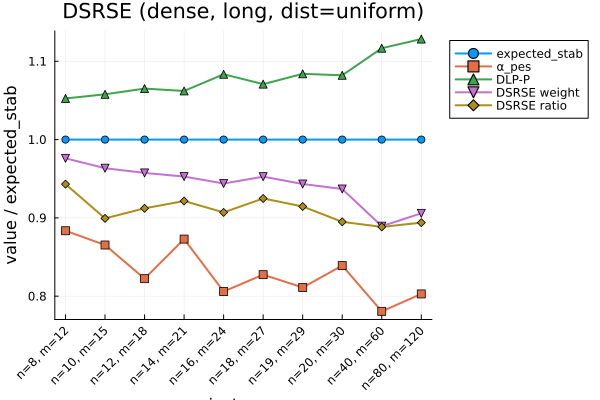
\includegraphics[width=\textwidth]{plot_dsrse_dense_long_uniform.png}
    \caption{DSRSE: intervals with uniform start and end times, long expected length and are densely packed across the slots.}
    \label{fig:DSRSE-Uni}
    \end{subfigure}
    \hfill
\begin{subfigure}[h]{0.49\textwidth}
        \centering
        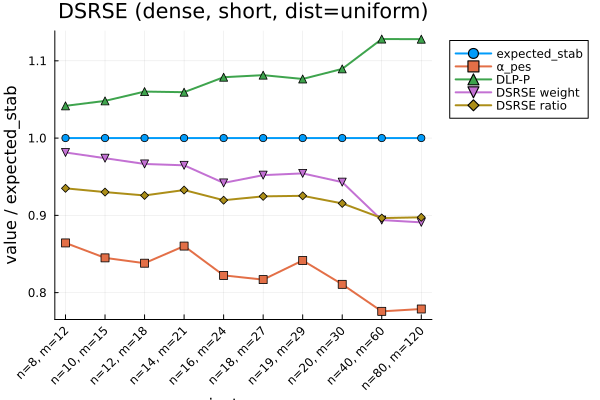
\includegraphics[width=\textwidth]{plot_dsrse_dense_short_uniform.png}
        \caption{DSRSE: intervals with uniform start and end times, short expected length and are densely packed across the slots.}
        \label{fig:DSRSE-Gau}
\end{subfigure}
    \begin{subfigure}[h]{0.49\textwidth}
    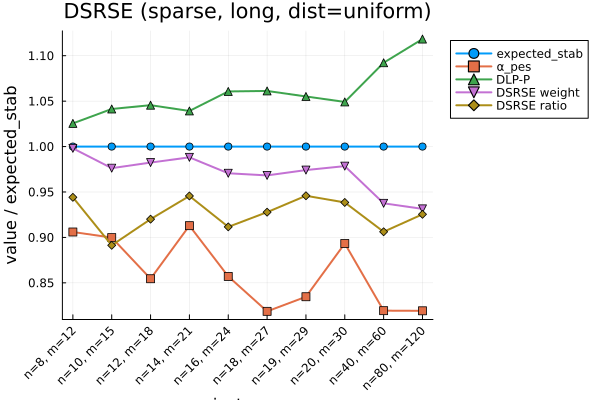
\includegraphics[width=\textwidth]{plot_dsrse_sparse_long_uniform.png}
    \caption{DSRSE: intervals with uniform start and end times, long expected length and are sparsely packed across the slots.}
    \label{fig:DSRSE-Uni}
    \end{subfigure}
    \hfill
\begin{subfigure}[h]{0.49\textwidth}
        \centering
        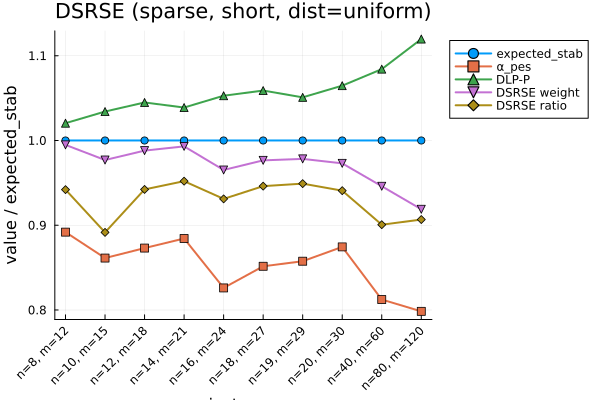
\includegraphics[width=\textwidth]{plot_dsrse_sparse_short_uniform.png}
        \caption{DSRSE: intervals with uniform start and end times, short expected length and are sparsely packed across the slots.}
        \label{fig:DSRSE-Gau}
\end{subfigure}
\caption{DSRSE}
        \label{fig:DSRSE}
\end{figure}

In Figure \ref{fig:DSRSE}, we present the value of each bound and heuristic on DSRSE instances after being normalized by the expected stability number.
DLP-P denotes the optimal value of~\eqref{DLP-P}, DSRSE-weight is the expected value of the greedy policy that schedules the largest-gained-weight task, and DSRSE-ratio is the expected value of the greedy policy that schedules the largest $w_i/\E[\text{length of }i]$; $\alpha_\pes$ denotes the optimal value of the pessimistic realization and expected\_stab denotes the expected stability number.
The \eqref{DLP-P} bound is slightly looser than the expected stability number for these instances, with performance gradually worsening as the instance size increases; on average, it is roughly $7\%$ above. 
We observe similar behavior for both heuristics; in addition, DSRSE-weight consistently outperforms DSRSE-ratio. On average, the former's gap is $4.5\%$ and the latter's is $8.9\%$. The pessimistic stability number, $\alpha_\pes$, has an average gap with the expected stability number of almost $16\%$.
%From the plots, we can see that DSRSE-weight and DSRSE-ratio are both close to the expected stability number under all four instance settings. 
%The optimal solution is lower bounded by DSRSE-weight, DSRSE-ratio and upper bounded by the expected stability number, so the two heuristics are practical in this case.
%By contrast, in the plots,~\eqref{DLP-P} is lower bounded by the expected stability number so it does not give a useful bound in this case.
%On average, the value of~\eqref{DLP-P}, $\alpha_\pes$, DSRSE-weight, DSRSE-ratio are $1.071718$, $0.840570$, $0.954901$, $0.917865$ respectively.

\begin{figure}[h]
    \centering
    \begin{subfigure}[h]{0.49\textwidth}
    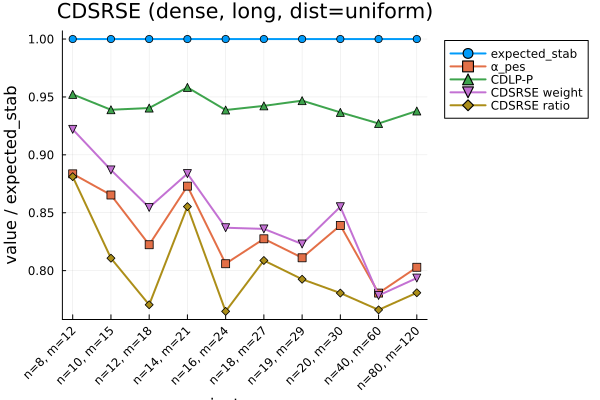
\includegraphics[width=\textwidth]{plot_cdsrse_dense_long_uniform.png}
    \caption{CDSRSE: intervals with uniform start and end times, long expected length and are densely packed across the slots.}
    \label{fig:CDSRSE-Uni}
    \end{subfigure}
    \hfill
\begin{subfigure}[h]{0.49\textwidth}
        \centering
        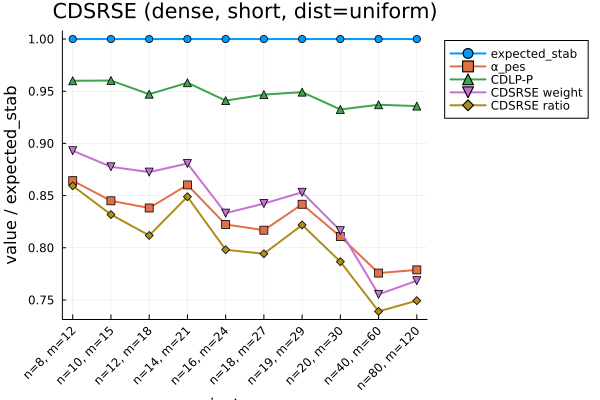
\includegraphics[width=\textwidth]{plot_cdsrse_dense_short_uniform.png}
        \caption{CDSRSE: intervals with uniform start and end times, short expected length and are densely packed across the slots.}
        \label{fig:CDSRSE-Gau}
\end{subfigure}
    \begin{subfigure}[h]{0.49\textwidth}
    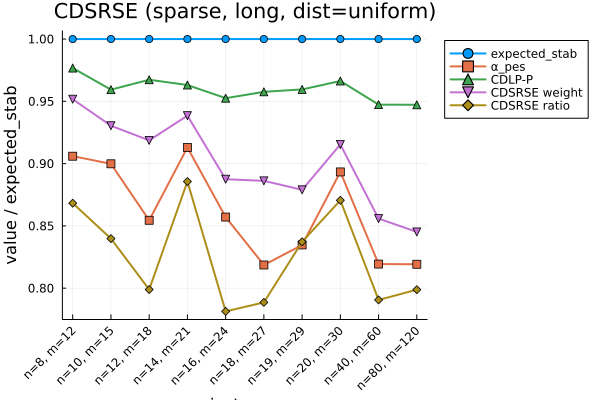
\includegraphics[width=\textwidth]{plot_cdsrse_sparse_long_uniform.png}
    \caption{CDSRSE: intervals with uniform start and end times, long expected length and are sparsely packed across the slots.}
    \label{fig:CDSRSE-Uni}
    \end{subfigure}
    \hfill
\begin{subfigure}[h]{0.49\textwidth}
        \centering
        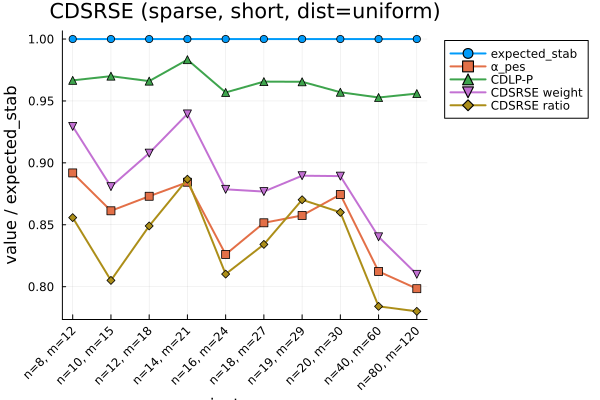
\includegraphics[width=\textwidth]{plot_cdsrse_sparse_short_uniform.png}
        \caption{CDSRSE: intervals with uniform start and end times, short expected length and are sparsely packed across the slots.}
        \label{fig:CDSRSE-Gau}
\end{subfigure}
\caption{CDSRSE}
        \label{fig:CDSRSE}
\end{figure}
Figure~\ref{fig:CDSRSE} presents analogous results for CDSRSE. % the value of each bound, heuristic after being normalized by the expected stability number.
In this case, the bound \eqref{CDLP-P} is uniformly better than the expected stability number, with values $5\%$ lower on average.
The heuristics do not perform as well because conflicts are enforced more conservatively in this model. DSRSE-weight is still usually superior to DSRSE-ratio, but the latter does better for the largest dense instances. The heuristics' average gaps with respect to \eqref{CDLP-P} are now $9\%$ and $14.7\%$.
%For CDSRSE, DSRSE-weight and DSRSE-ratio do not perform as well because conflicts are enforced conservatively. 
%Even though the LP relaxation~\eqref{CDLP-P} provides lower bounds close to the expected stability number, we do not know its actual performance since both are upper bounds for CDSRSE.
%In this case, the gaps between~\eqref{CDLP-P} and the heuristics are better indicator of the estimation errors.
%On average, the value of~\eqref{CDLP-P}, $\alpha_\pes$, DSRSE-weight, DSRSE-ratio are $0.950845$, $0.840570$, $0.864773$, $0.810323$ respectively.


\bibliographystyle{siam}
\bibliography{SDPVFA}

\end{document}
